\section{Defect mechanisms and optical quality}
\label{sec:defects}
\subsection{A transparent object is not necessarily an imaging optic}
Optical qualification should separate total transmission, directional transmission, wavefront quality, and scattering. A ribbed transparent wall can transmit considerable light while producing strong image distortion. Conversely, a deliberately patterned illumination element may use that distortion productively. The early G3DP work demonstrates transparent structures and controllable caustic patterns; it is not evidence that an as-printed wall has the surface figure of a polished lens.\cite{acad_klein2015}

Destino and colleagues provide a different benchmark: silica and silica--titania glasses prepared by sol--gel-derived ink writing followed by thermal processing were characterized against commercial optical glasses. Their work includes polished surfaces and refractive-index homogeneity, so those results should not be attributed to as-deposited molten cords.\cite{acad_destino2018} Cross-route comparisons need the whole process history, including polishing, thermal densification, coatings, and measurement path length.

\subsection{Mechanism-based diagnosis}
Entrained gas, inter-track voids, crystalline inclusions, foreign particles, and surface damage can all reduce performance but demand different remedies. Gas already in a reservoir calls for feedstock and conditioning investigation. Voids recurring at junctions suggest deposition geometry or insufficient bonding. A rough surface can arise from layer shape without implying bulk porosity. Crystals require phase-sensitive characterization; their presence must not be inferred from every bright spot in a microscope image.

Devitrification depends on composition, nucleation sites, temperature, and exposure time. A liquidus temperature describes an equilibrium phase boundary, not a complete kinetic guarantee that a print remains amorphous. Recommended characterization includes differential scanning calorimetry at stated heating rates, diffraction, and microscopy after representative thermal cycles. Recycling further demands chemical identity and contamination checks. Mixing individually transparent cullets does not establish thermal compatibility or a common viscosity curve. These are proposed qualification measures, not claims that the cited recycled-glass study demonstrated every test.

For optical loss, a basic homogeneous attenuation model is
\begin{equation}
 T_{\mathrm{int}}(\lambda,d)=\exp[-\mu(\lambda)d].
\end{equation}
External transmission also includes interface reflections, collection geometry, and scattering. For a simple plane-parallel transparent specimen, surface reflection losses cannot be silently assigned to bulk absorption. Reporting a single percentage without wavelength, thickness, surface condition, and whether scattered light is collected is insufficient for ranking processes. Likewise, roughness $R_a$ is a profile statistic at a stated cutoff and direction; it does not alone specify optical wavefront quality.

\subsection{Interlayer bonding and mechanical evidence}
The KTH filament study measured both line geometry and bonding width, providing evidence that deposited width and actual contact width need not be equal. Its multilayer results demonstrate reproducible bonding under the selected operating conditions, not an independently measured universal tensile strength.\cite{acad_liu2022} A visible line in a transparent print may represent surface geometry, an internal interface, compositional variation, or stress; fracture analysis is needed to identify the feature that actually controls failure.

A 2026 study by Chhadeh and colleagues directly addresses mechanical performance of extruded soda-lime glass. Its four-point bending experiments show dependence on toolpath and layer orientation and connect performance to thermal retention during deposition. The reported $90^\circ$ specimens had mean strength approximately 40\% greater than the $0^\circ$ specimens in that experiment. This is a within-study comparison, not a transferable design factor. The test setup deliberately differs from EN~1288-3 in dimensions and roller freedom; it should not be described as unqualified standard conformity.\cite{acad_chhadeh2026}

The engineering implication is that orientation labels alone are inadequate predictors: they can also change path length, return time, and the heat history of adjacent tracks. A proposed experimental design should hold those factors separately where possible and record specimen surface treatment, effective loaded area, loading rate, environment, and failure origin. Report the specimen count and full strength distribution rather than the strongest coupon. Comparing flexural strength with direct tensile strength, or comparing specimens with different flaw populations, can obscure the actual process improvement.

\subsection{Polarimetry and an application-specific acceptance chain}
\begin{figure}[htbp]\centering
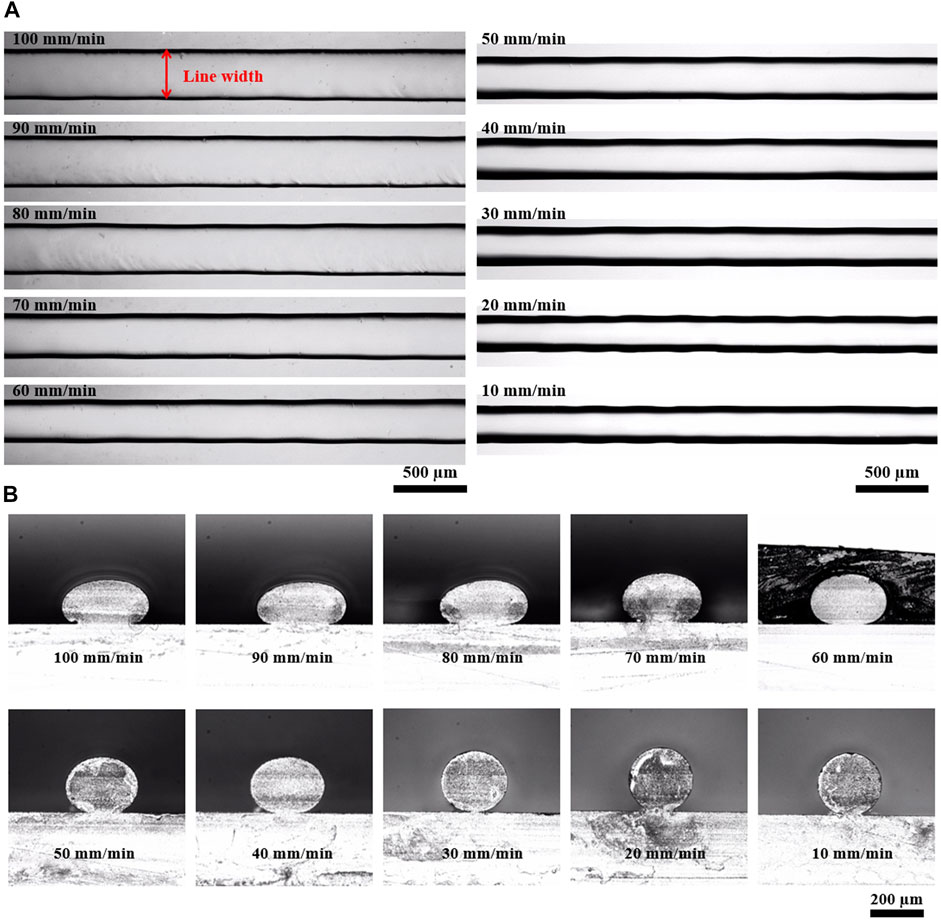
\includegraphics[width=.8\linewidth]{figures/Liu2022_Figure6.jpg}
\caption{Top views and cross-sections of deposited silica lines for travel speeds of 10--100 mm/min and laser powers specified in the original experiment. The figure supports comparison of contact geometry; it is not a generic bubble or residual-stress image. Liu, Oriekhov and Fokine (2022), Figure 6, reproduced unmodified from \href{https://doi.org/10.3389/fmats.2022.978861}{the primary paper} under \href{https://creativecommons.org/licenses/by/4.0/}{CC BY 4.0}.}
\end{figure}
In a simple uniform, plane-stress specimen with fixed principal directions, optical retardation can be written
\begin{equation}
 \delta=C(\lambda,T)(\sigma_1-\sigma_2)d.
\end{equation}
The stress-optic coefficient $C$ is material and wavelength dependent. For a spatially varying field, the interpretation is path dependent; curved surfaces and changing principal directions complicate inversion. SCHOTT describes the relationship between stress birefringence and optical performance.\cite{acad_schott2023} A colorful crossed-polarizer photograph is a useful screening observation, but it is not by itself a calibrated three-dimensional stress map. Darkness can also result from an unfavorable orientation rather than the absence of stress.

This review proposes an acceptance chain tied to intended service: first geometry and surface inspection; then bulk void/inclusion checks; then optical transmission and, where needed, wavefront or haze; then calibrated residual-stress assessment; finally mechanical tests on representative specimens and connections. Hermetic fluidics additionally require pressure and leak testing; decorative lighting requires a different optical specification from an imaging lens. Passing one branch does not certify another. This approach turns the broad word ``transparent'' into measurable requirements while preserving the possibility that intentional texture, color, or scattering is useful product functionality.

\begin{figure}[htbp]\centering
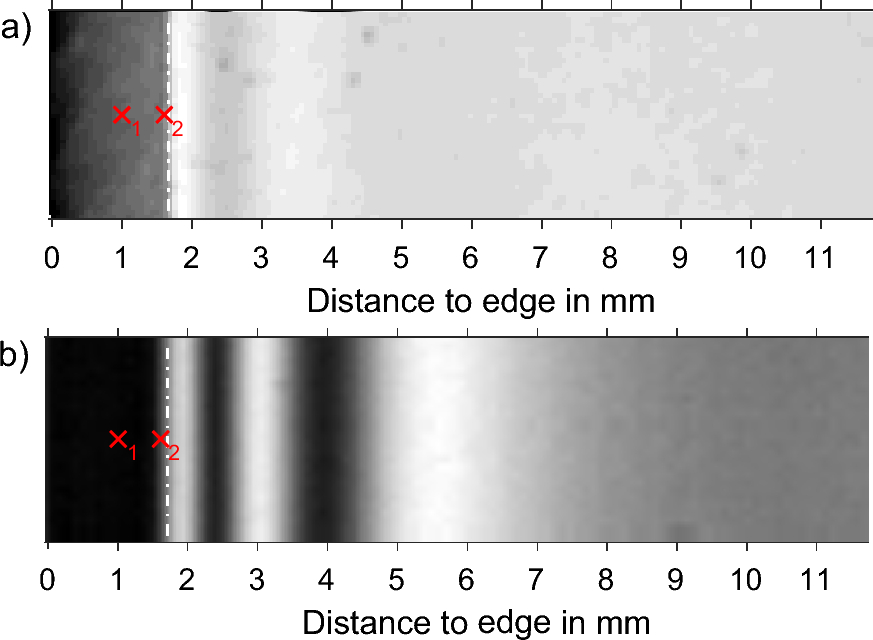
\includegraphics[width=.8\linewidth]{figures/Efferz2024_Figure2.png}
\caption{Measurement-method illustration using conventional fully tempered glass, \emph{not a printed specimen}. Intensity and isochromatic images near the edge of a 10 mm specimen; marked positions are approximately 1.0 and 1.6 mm from the edge, and the dashed line identifies the chamfer. Efferz, Schuler and Siebert (2024), Figure 2, reproduced unmodified from \href{https://doi.org/10.1007/s40940-024-00270-3}{the primary article} under \href{https://creativecommons.org/licenses/by/4.0/}{CC BY 4.0}.}
\end{figure}
